\documentclass[11pt,a4paper,toc=bibliography,toc=listof,titlepage=firstiscover]{scrreprt}
\usepackage[utf8]{inputenc}
\usepackage{blindtext}
\usepackage{graphicx}
\usepackage{subcaption}
\usepackage[T1]{fontenc}
\usepackage{setspace}
\usepackage{pdfsync}
\usepackage{blindtext}
\usepackage[ngerman]{babel}
\usepackage{booktabs}
\usepackage{xcolor}
\usepackage{multirow}
%Schriftarten hier definieren
\usepackage{lmodern}
%\usepackage{tgheros}
%\renewcommand*\familydefault{\sfdefault}
%\usepackage{tgpagella}
\usepackage[babel,german=guillemets]{csquotes}
\usepackage[style=apa]{biblatex}
\usepackage{hyperref}
\usepackage{csquotes}
\addbibresource{resources/literatur.bib}
\hypersetup{colorlinks=true, linkcolor=black, urlcolor=black, citecolor=black}
%Abstand der Einträge im Literaturverzeichnis als em
\setlength\bibitemsep{0.75em}
%Kein Einzug bei einem neuen Absatz
\setlength{\parindent}{0mm}
%Inhaltsverzeichnis ohne eigene Seitenzahl
\AtBeginDocument{\addtocontents{toc}{\protect\thispagestyle{empty}}} 
\usepackage[left=3cm,right=2.5cm,top=2.5cm,bottom=2cm]{geometry}

%Daten des Deckblatts
  \titlehead
  {
    {
      \begin{center}
        \vspace{2.5cm}
        
\includegraphics[scale=0.3]{resources/nak-logo.png}
      \end{center}
    }
  	%M.Sc. Angewandte Informatik
  }
  \subject{Hausarbeit}
  \title{Integration der Data Science in Organisationen / Abteilungen}
    \subtitle{Vorlesung Data-Science Projektorganisation}
    \author{Leon Henne}
  \date{\small{Köln, den \today}}
  \publishers{Betreut durch Prof. Dr. Michael Schulz}
\begin{document}
%Titelseite erzeugen
\maketitle
%Der Nachfolgende Text wird 1,5-zeilig gesetzt
\onehalfspacing
%Römische Ziffern für Abbildungsverzeichnis
\pagenumbering{Roman}
\setcounter{page}{0}
%Inhaltsverzeichnis erzeugen
\tableofcontents
\clearpage
%Abbildungs und Tabellenverzeichnis
\listoftables
\listoffigures
%ToDo --> Abkürzungsverzeichnis
\clearpage
\pagenumbering{arabic}
\setcounter{page}{1}
%Datei aus dem Ordner /chapter/ einbinden. So kann man mehrere Textdateien zu einem großen Dokument zusammenfügen.
\setcounter{chapter}{0}

\chapter[Problemstellung]{Problemstellung}

Viele Trends der technologischen Welt innerhalb der letzten Jahrzehnte wurden besonders durch drei bestimmende Faktoren beeinflusst.
Die Entwicklung der Datenspeicherungs- und Rechenkapazitäten als zwei dieser Faktoren entstammen den Erkenntnissen und sich bestätigenden Entwicklungen von Gorden E. Moore bzw. dem Moorschen Gesetz. \footcite[Vgl.][S. 1]{Moore.1998}
Demnach wurde bereits sehr früh erkannt, dass integrierte Schaltungen die bekannten Telefonschaltungen ersetzen wird und Computer leistungsfähiger entsprechende Daten verarbeiten können. \footcite[Vgl.][S. 1]{Moore.1998}
Erkenntlich wird diese Entwicklung anhand der heutzutage konstanten und umfangreichen Generierung von Daten durch Anwendungen in Mobiltelefonen, Autos, IOT Geräten oder Industriemaschinen. \footcite[Vgl.][S 3f.]{Dalpiaz.2020}
Prognosen sagen dabei eine verfünffachende Entwicklung der globalen Datenmenge vorher von 33 Zettabytes in 2018 zu 175 Zettabytes in 2025. \footcite[Vgl.][S. 1]{Hupperz.2021}
Der dritte Faktor ist die Entwicklung der Möglichkeiten zur Datenverarbeitung und Analyse anhand von zunehmend komplexeren Algorithmen. \footcite[Vgl.][S. 4]{Dalpiaz.2020}

Folgend aus diesen drei Faktoren zielen immer mehr Software Unternehmen darauf ab, sich in eine datengesteuerte Organisation zu transformieren. \footcite[Vgl.][S. 1]{Fabijan.2017}
Höheres Interesse an dem Besitz und der Verarbeitung großer Datenmengen zeigen heutzutage jedoch Organisationen aller Bereiche wie Wirtschaft, Regierungen und Forschung. \footcite[Vgl.][S. 1]{Pratt.2023}
Deren Stratgien weisen häufig auf, mittels datenfokussierter Kultur und Datenanalysen möglichst umfangreiche faktenbasierte Entscheidungen zu treffen. \footcite[Vgl.][S. 18]{Dalpiaz.2020}
Forschungsfeld dieser Absicht bildet die Data Science, bzw. Big Data Analytics mit dessen Einsatz von Technologien sich Unternehmen einen Wettbewerbsvorteil erzielen. \footcite[Vgl.][S. 3]{Dalpiaz.2020}
datengesteuerte Unternehmen können dadurch bis zu 26 \% profitabler werden gegenüber Wettbewerbern, welche weniger bis gar keine digitalen Technologien einsetzen. \footcite[Vgl.][S. 1]{Fabijan.2017}
Ein Grund dafür können bessere und schnellere Entscheidungen sein, welche aus dem vollumfänglicheren Verständnis des Kunden und höherer Transparenz des Entwicklungsprozesses resultieren. \footcite[Vgl.][S. 18]{Dalpiaz.2020}
Trotz der heute vorhandenen Fülle von erzeugten Daten bleibt die Anzahl an Unternehmen, welche erfolgreich in eine datengesteuerte Organisation transformierten eher gering. \footcite[Vgl.][S. 1]{Fabijan.2017}
Zusätzlich existiert bisher nur wenig Forschung dazu, wie solche Transformationen zu datengesteuerte Unternehmen umzusetzen sind. \footcite[Vgl.][S. 1]{Fabijan.2017}

% \begin{itemize}
%     \item Entwicklung von Datenspeicherung, Rechenpower und Analysemöglichkeiten
%     \item Relevanz der Thematik für Organisationen als Wettbewerbsvorteil (was bringt es ?) 
%     \begin{itemize}
%         \item Steigende Notwendigkeit der Integration von Data Science zur Marktpositionierung
%     \end{itemize}
%     \item Aktualität des Problems (Bisher hat es halt keiner gemacht)
% \end{itemize}
\chapter[Grundlagen]{Grundlagen}

\section{Disziplin der Data Science}



\section{Organisationen}

\section{Abgrenzung von Daten getriebenen Organisationen}
\chapter{Data Science in datengesteuerten Organisationen}

Inhalt dieses Kapitels ist die Darstellung des aktuellen Stands der Forschung zur Eingliederung von Data Science Teams in datengesteuerten Organisationen.
Damit wird verfolgt, ein aktuelles Zielbild annäherungsweise zu konkretisieren, um in weiteren Kapiteln auf die Möglichkeiten zur Integration einzugehen.

Eine Herausforderung entsteht bereits dabei, dass datengesteuerte Organisationen, in der Fachsprache als \textit{data driven Organizations} bezeichnet, einer Vielfalt an Definitionen unterliegen. \footcite[prenote][postnote]{(several definitons of DDOs)}
\Citeauthor*{Fabijan.2017} definierte z. B., dass datengesteuerte Organisationen Daten akquirieren, verarbeiten und Datenvorteile in einer zeitlich angebrachten Art und Weise nutzen, um Effizienzgewinne zu erzeugen, neuartige Produkte zu entwickeln und sich durch die Wettbewerbslandschaft zu navigieren. \footcite[prenote][postnote]{DDO definition}
% insert second definition
Ein gemeinsames Verständnis der Definitionen besteht in dem Prozess des Sammeln von Daten, der Gewinnung von Erkenntnissen durch Analysen und dem Treffen von Entscheidungen basierend auf den erzielten Analyseergebnissen. \footcite[prenote][postnote]{looking into DDO definitions}

Einer der wichtigsten Aspekte einer datengesteuerten Organisation ist die Manifestation einer datengesteuerten Kultur. \footcite[prenote][postnote]{data-driven culture}
Dessen Antrieb ist es, Daten nicht nur den Analytic-Abteilungen oder dem leitenden Management vorbehalten sind, sondern so weit wie rechtlich möglich, jedem Organisationsmitglied zur Verfügung gestellt werden sollte. \footcite[prenote][postnote]{ddos democratize data}
Dieser Umgang würde es ermöglichen, alle Arten der Analyse (deskriptiv, prädiktiv, präskriptiv) auf allen Ebenen der Organisation (operativ, taktisch, strategisch) einzusetzen. \footcite[prenote][postnote]{typees of analytics}
In der bisherigen Praxis wird von diesen Möglichkeiten jedoch nur ein Teil angewendet. \footcite[prenote][postnote]{typees}
Weitere Aspekte einer datengesteuerten Organisation konnten durch die Forschung von \Citeauthor*{Marius Hupperz, Inan Gür et al. 2021} identifiziert werden.
Für den untersuchten Aspekt der Data Science ist erkannt worden, dass der Wertbeitrag durch Transparenz, zielgerichtetem Marketing oder automatisierten informierten Entscheidungen zu Wettbewerbsvorteilen führen kann, jedoch keinen unmittelbaren Einflüsse auf die Vermögenswerte ausüben. \footcite[prenote][postnote]{data science brings value}
Zusätzlich kann Einrichtung einer Digitalisierungsabteilung zwar die Transformation zum datengesteuerten Unternehmen unterstützen, jedoch durch das alleinige Einrichten von Data Science Abteilungen keine Geschäftserkenntnisse aus Daten zu erzeugen. \footcite[prenote][postnote]{data science teams}
Alle weiteren Aspekte aus der strukturierten Literaturanalyse von datengesteuerten Organisationen sind in folgender Abbildung 3.1 dargestellt:

\begin{figure}[htb]
    \centering
    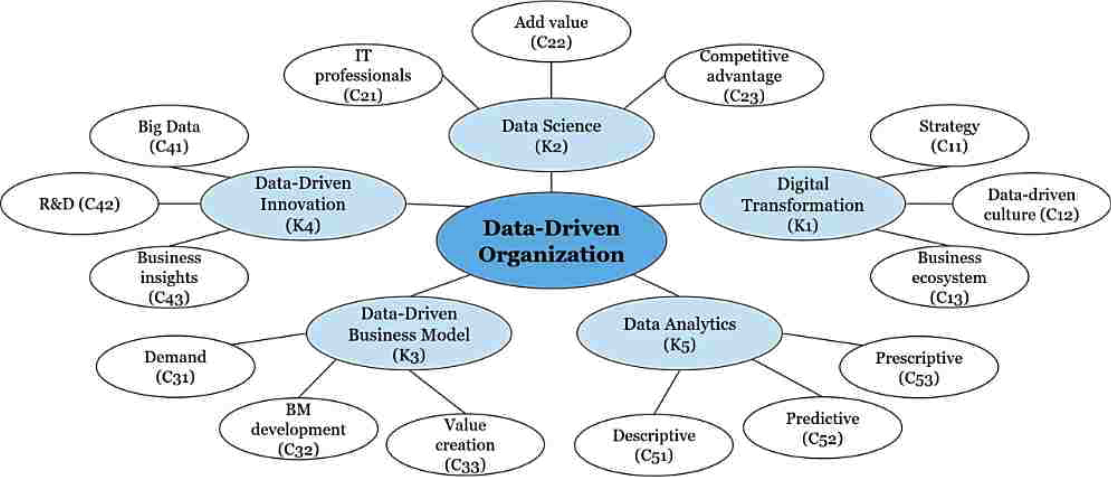
\includegraphics[width=0.95\textwidth]{graphics/ddo aspects.png}
    \caption{In der Literatur beschriebene Aspekte von datengesteuerten Organisationen}
    \label{fig:DDOs aspects}
\end{figure}

Zur praktischen Umsetzung von datengesteuerten Unternehmen führten \Citeauthor*{Zhang, Muller et al. 2020} eine Online Befragung mit insgesamt 183 Teilnehmenden aus der Data Science durch.
Da alle Beteiligten der Umfrage aus dem IT-Konzern IBM stammen, ist die Umfrage zwar nicht statistisch repräsentativ für alle Organisationen, zeigt jedoch ein signifikantes Bild über den Aufbau und die Zusammenarbeit von Data Science Abteilungen.
Mit der Umfrage sind Erkenntnisse sind erzielt worden, die fachliche, personelle und rollenbezogene Zusammensetzung und Zusammenarbeit von Data Science Abteilungen betreffen.
Ein Ergebnis der Umfrage ist es, dass Data science Abteilungen häufig mit einer Teamgröße von bis zu sechs Personen arbeiten, wobei jede Person bis zu 5 Jahre Erfahrung mit Data Science Projekten aufweisen kann. \footcite[prenote][postnote]{(histogram of data science)}
Dabei führen die Teammitglieder meistens mehr als eine Rolle aus, was aus der nachträglichen Abbildung \textbf{X} hervorgeht: \footcite[prenote][postnote]{(histogram2x of data science)}

\begin{figure}[h]
    \centering
    \begin{subfigure}[b]{0.45\textwidth}
      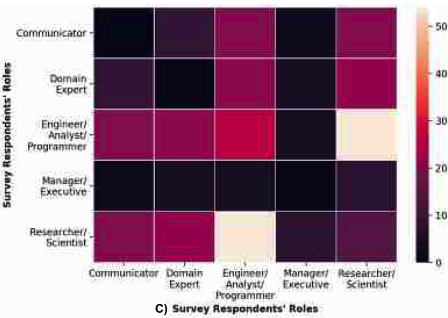
\includegraphics[width=\textwidth]{graphics/ds team roles.png}
      \caption{Häufigkeit der gemeinsam auftretenden Rollen in Data Science Teams}
      \label{fig:heatmap roles}
    \end{subfigure}
    \hfill
    \begin{subfigure}[b]{0.45\textwidth}
      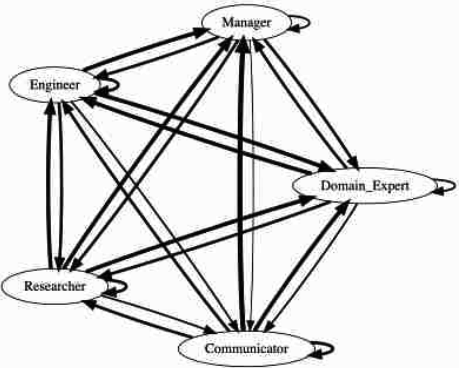
\includegraphics[width=\textwidth]{graphics/ds team network .png}
      \caption{Beziehungsgraph der Zusammenarbeit einzelner Rollen in Data Science Teams}
      \label{fig:network graph}
    \end{subfigure}
    \caption{Rollen und deren Zusammenarbeit in Data Science Teams}
    \label{fig:both_figures}
\end{figure}

Aus der Heatmap wird deutlich, dass die Kombination der Rollen \textit{Researcher - Engineer} am Häufigsten auftritt.
Dies resultiert vermutlich daraus, dass sich in der recht jungen Disziplin der Data Science noch wenig Standards etablierten, wodurch viele Konzepte in Projekten erstmalig zu entwickeln sind.
Durch die Diagnole der Abbildung, in welcher die Häufigkeit von einzeln vorkommenden Rollenbesetzungen abgetragen ist, wird ersichtlich, dass die \textit{Engineer} Rolle häufiger als alle anderen von einer Person ausgefüllt wird.
Daraus lässt sich vermuten, dass der hohe Entwicklungsaufwand in Data Science Projekten die Fokussierung von Personal zur \textit{Engineer} Rolle rechtfertigt.
Als Person in der Rolle des Managers werden, mit Ausnahme der \textit{Researcher} Rolle, noch seltener weitere Rollen ausgeübt, jedoch auch selten lediglich Aufgaben der eigenen Rolle übernommen.
Begründbar erscheint dies durch die Annahme, dass das Management häufig Aufgaben außerhalb des direkten Geschehens im Data Science Projekt umfasst.
Die Ausnahme der \textit{Researcher} Rolle würde sich logisch durch den gemeinsamen hohen Bedarf an Arbeitserfahrung im Themenfeld begründen lassen.

Abbildung \textbf{X} zeigt den Umfang der Zusammenarbeit zwischen den verschiedenen Rollen auf.
Auffälligkeiten in der Grafik umfassen die Rolle des \textit{Communicators} und des \textit{Domain Experts}.
Die Rolle des \textit{Communicators} wird dabei vermutlich häufig sehr extrovertiert gestaltet, da hier besonders viel ausgehende Zusammenarbeit zu den anderen Rollen erkennbar ist, im Vergleich zu dessen Abhängigkeit.
Etwas gegensätzlich dazu zeigt sich die Rolle des \textit{Domain Experts}, welcher eine starke Abhängigkeit anderer Rollen abbildet, obwohl dabei wesentlich weniger technische Expertise zu erwarten ist.

% anschließend die Collaboration Points anbringen
In datengesteuerten Organisationen gilt es für eine Data Science Abteilung nicht nur innerhalb von sich selbst zusammenzuarbeiten, sondern auch z. B. Komponenten für maschinelles Lernen mit anderen Softwareabteilungen nutzbar zu gestalten.
Dazu sind vielerlei Punkte in der Abstimmung beider Teams notwendig, wie bspw. Anforderungserhebung, Trainingsdaten und Modellintegration, welche nachfolgend detaillierter betrachtet werden.

\chapter[Integrationsprozesse]{Integrationsprozesse}

Anschließend an die Beschreibung einer datengesteuerten Organisation, dessen Aufbau, Prozesse und Rollen werden innerhalb dieses Kapitels die Herausforderungen und Vorgehenswege zur Transformation in eine datengesteuerte Organisation thematisiert.

\section{Herausforderungen}

Bereits aus dem Zielbild, datengesteuert Entscheidungen in Organisation zu treffen (z.B. zur Strategie), ergibt sich die Herausforderung, Entscheidungen hohen Ausmaßes in sich schnell wechselnden kompetitiven Umgebungen auszuführen. \footcite[Vgl.][S. 2]{Pratt.2023} 
Hinzu zu der Geschwindigkeit der Geschäftsumgebung, konnte durch eine Gartner Umfrage festgestellt werden, dass 65 \% der Teilnehmenden im Zeitraum der letzten zwei Jahre (2021-2023) einen Zuwachs in der Komplexität der Entscheidungen verzeichneten. \footcite[Vgl.][S. 65]{Pratt.2023}

Daraus resultierend zeigt sich, dass vor allem managementbezogene und kulturelle Herausforderungen die Transformation beeinflussen, neben den ohnehin bestehenden technischen Hürden. \footcite[Vgl.][S. 15]{Dalpiaz.2020}
% Diese Herausforderungen bilden dabei jedoch recht umfassend die notwendigen Aspekte zur 

\begin{itemize}
    \item outside view (fast and complex decisions)
    \item manageral and cultural challenges
    \item technical challenges
    \item need for DS framework
\end{itemize}

\section{Vorgehensmodelle zur Integration von Data Science}

\begin{itemize}
    \item Conceptual requirements
    \item Design Parameters
    \item Experiment Evolution Model (Microsoft)
    \item CSPG Framework
    \item DI / DS Integration Framework
\end{itemize}
\chapter[Betrachtung von Fallstudien]{Betrachtung von Fallstudien}
\chapter[Fazit]{Fazit}
Ziel dieser Arbeit war die Beleuchtung der aktuellen Forschungsliteratur zur Integration von Data Science in Organisationen und Abteilungen.
Dazu wurde zunächst ein Grundlagenverständnis der Data Science geschaffen und das Zielbild einer datengesteuerten Organisation thematisiert.
Anschließend wurde im Detail auf die Herausforderungen der Integration eingegangen.
Folgend wurden aus der Forschungsliteratur verschiedene Modelle zur Transformation in eine datengesteuerte Organisation und dessen Gestaltung dargelegt.

Durch die Hausarbeit konnte verdeutlicht werden, welche Auswirkung eine Integration der Data Science im Unternehmen erzeugen kann, jedoch auch, wie herausfordernd und aufwändig eine Transformation zur datengesteuerten Organisation ist.
Als Disziplin, um aus Daten Mehrwerte zu generieren kann die Data Science in datengesteuerten Organisationen Prozesse verbessern, transparentere Entscheidungsgrundlagen schaffen und Innovationen fördern.
Externe Faktoren, wie das sich schnell verändernde Umfeld und interne Herausforderungen, wie die Datenkultur, das Vertrauen in Daten und fehlende IT-Infrastruktur erschweren jedoch die Integration der Data Science.
In der Forschung wurden daher verschiedene Modelle entwickelt, um die Integration phasenweise zu begleiten, oder das Zielbild in leichter umzusetzende Teilaspekte aufzugliedern. 

Zusammenfassend lässt sich erkennen, dass die Integration der Data Science in Organisation eine wichtige Aufgabe für alle Teile der Gesellschaft wie Wirtschaft, Politik und Forschung geworden ist.
Daher sollten alle Gesellschaftsbereiche mit Best Practices, Bildungsmaßnahmen und ausgiebiger Forschung zur Bewältigung dieser Aufgabe beitragen.

%Literaturverzeichnis einfügen
\renewcommand*{\UrlFont}{\rmfamily}
\printbibliography
\include{chapter/99_eidesstattliche-erkläerung.tex}
\end{document}
